\documentclass{article}

\usepackage[utf8]{inputenc}
\usepackage{fullpage}
\usepackage{amsmath, amssymb, amsfonts, amsthm}
\usepackage{bbm}
\usepackage{mathtools}
\usepackage{twoopt}
\usepackage{babel}
\usepackage{tikz}
\usepackage{enumitem}

\def \lastexercisenumber {0}

% special letters:

\newcommand{\N}{\mathbb{N}}
\newcommand{\Z}{\mathbb{Z}}
\newcommand{\Q}{\mathbb{Q}}
\newcommand{\R}{\mathbb{R}}
\newcommand{\C}{\mathbb{C}}
\newcommand{\K}{\mathbb{K}}
\newcommand{\T}{\mathbb{T}}
\newcommand{\E}{\mathbb{E}}
\newcommand{\V}{\mathbb{V}}
\renewcommand{\S}{\mathbb{S}}
\renewcommand{\P}{\mathbb{P}}
\newcommand{\1}{\mathbbm{1}}

% quantors:

\newcommand{\Forall}{\forall \,}
\newcommand{\Exists}{\exists \,}
\newcommand{\ExistsOnlyOne}{\exists! \,}
\newcommand{\nExists}{\nexists \,}
\newcommand{\ForAlmostAll}{\forall^\infty \,}

% MISC symbols:

\newcommand{\landau}{{\scriptstyle \mathcal{O}}}
\newcommand{\Landau}{\mathcal{O}}


\newcommand{\eps}{\mathrm{eps}}

% graphics in a box:

\newcommandtwoopt
{\includegraphicsboxed}[3][][]
{
  \begin{figure}[!h]
    \begin{boxedin}
      \ifthenelse{\isempty{#1}}
      {
        \begin{center}
          \includegraphics[width = 0.75 \textwidth]{#3}
          \label{fig:#2}
        \end{center}
      }{
        \begin{center}
          \includegraphics[width = 0.75 \textwidth]{#3}
          \caption{#1}
          \label{fig:#2}
        \end{center}
      }
    \end{boxedin}
  \end{figure}
}

% braces:

\newcommand{\pbraces}[1]{{\left  ( #1 \right  )}}
\newcommand{\bbraces}[1]{{\left  [ #1 \right  ]}}
\newcommand{\Bbraces}[1]{{\left \{ #1 \right \}}}
\newcommand{\vbraces}[1]{{\left  | #1 \right  |}}
\newcommand{\Vbraces}[1]{{\left \| #1 \right \|}}
\newcommand{\abraces}[1]{{\left \langle #1 \right \rangle}}
\newcommand{\round}[1]{\bbraces{#1}}

\newcommand
{\floorbraces}[1]
{{\left \lfloor #1 \right \rfloor}}

\newcommand
{\ceilbraces} [1]
{{\left \lceil  #1 \right \rceil }}

% special functions:

\newcommand{\norm}  [2][]{\Vbraces{#2}_{#1}}
\newcommand{\diam}  [2][]{\mathrm{diam}_{#1} \: #2}
\newcommand{\diag}  [1]{\mathrm{diag} \: #1}
\newcommand{\dist}  [1]{\mathrm{dist} \: #1}
\newcommand{\mean}  [1]{\mathrm{mean} \: #1}
\newcommand{\erf}   [1]{\mathrm{erf} \: #1}
\newcommand{\id}    [1]{\mathrm{id} \: #1}
\newcommand{\sgn}   [1]{\mathrm{sgn} \: #1}
\newcommand{\supp}  [1]{\mathrm{supp} \: #1}
\newcommand{\arsinh}[1]{\mathrm{arsinh} \: #1}
\newcommand{\arcosh}[1]{\mathrm{arcosh} \: #1}
\newcommand{\artanh}[1]{\mathrm{artanh} \: #1}
\newcommand{\card}  [1]{\mathrm{card} \: #1}
\newcommand{\Span}  [1]{\mathrm{span} \: #1}
\newcommand{\Aut}   [1]{\mathrm{Aut} \: #1}
\newcommand{\End}   [1]{\mathrm{End} \: #1}
\newcommand{\ggT}   [1]{\mathrm{ggT} \: #1}
\newcommand{\kgV}   [1]{\mathrm{kgV} \: #1}
\newcommand{\ord}   [1]{\mathrm{ord} \: #1}
\newcommand{\grad}  [1]{\mathrm{grad} \: #1}
\newcommand{\ran}   [1]{\mathrm{ran} \: #1}
\newcommand{\graph} [1]{\mathrm{graph} \: #1}
\newcommand{\Inv}   [1]{\mathrm{Inv} \: #1}
\newcommand{\pv}    [1]{\mathrm{pv} \: #1}
\newcommand{\GL}    [1]{\mathrm{GL} \: #1}
\newcommand{\Mod}{\mathrm{Mod} \:}
\newcommand{\Th}{\mathrm{Th} \:}
\newcommand{\Char}{\mathrm{char}}
\newcommand{\At}{\mathrm{At}}
\newcommand{\Ob}{\mathrm{Ob}}
\newcommand{\Hom}{\mathrm{Hom}}
\newcommand{\orthogonal}[3][]{#2 ~\bot_{#1}~ #3}
\newcommand{\Rang}{\mathrm{Rang}}
\newcommand{\NIL}{\mathrm{NIL}}
\newcommand{\Res}{\mathrm{Res}}
\newcommand{\lxor}{\dot \lor}
\newcommand{\Div}{\mathrm{div} \:}
\newcommand{\meas}{\mathrm{meas} \:}

% fractions:

\newcommand{\Frac}[2]{\frac{1}{#1} \pbraces{#2}}
\newcommand{\nfrac}[2]{\nicefrac{#1}{#2}}

% derivatives & integrals:

\newcommandtwoopt
{\Int}[4][][]
{\int_{#1}^{#2} #3 ~\mathrm{d} #4}

\newcommandtwoopt
{\derivative}[3][][]
{
  \frac
  {\mathrm{d}^{#1} #2}
  {\mathrm{d} #3^{#1}}
}

\newcommandtwoopt
{\pderivative}[3][][]
{
  \frac
  {\partial^{#1} #2}
  {\partial #3^{#1}}
}

\newcommand
{\primeprime}
{{\prime \prime}}

\newcommand
{\primeprimeprime}
{{\prime \prime \prime}}

% Text:

\newcommand{\Quote}[1]{\glqq #1\grqq{}}
\newcommand{\Text}[1]{{\text{#1}}}
\newcommand{\fastueberall}{\text{f.ü.}}
\newcommand{\fastsicher}{\text{f.s.}}

% -------------------------------- %
% amsthm-stuff:

\theoremstyle{definition}

% numbered theorems
\newtheorem{theorem}{Satz}
\newtheorem{lemma}{Lemma}
\newtheorem{corollary}{Korollar}
\newtheorem{proposition}{Proposition}
\newtheorem{remark}{Bemerkung}
\newtheorem{definition}{Definition}
\newtheorem{example}{Beispiel}

% unnumbered theorems
\newtheorem*{theorem*}{Satz}
\newtheorem*{lemma*}{Lemma}
\newtheorem*{corollary*}{Korollar}
\newtheorem*{proposition*}{Proposition}
\newtheorem*{remark*}{Bemerkung}
\newtheorem*{definition*}{Definition}
\newtheorem*{example*}{Beispiel}

% Please define this stuff in project ("main.tex"):

% \def \lastexercisenumber {...}
% This will be 0 by default

% \setcounter{section}{...}
% This will be 0 by default
% and hence, completely ignored

\ifnum \thesection = 0
{\newtheorem{exercise}{Aufgabe}}
\else
{\newtheorem{exercise}{Aufgabe}[section]}
\fi

\ifdef
{\lastexercisenumber}
{\setcounter{exercise}{\lastexercisenumber}}

\newcommand{\solution}
{
    \renewcommand{\proofname}{Lösung}
    \renewcommand{\qedsymbol}{}
    \proof
}

\renewcommand{\proofname}{Beweis}

% -------------------------------- %
% environment zum einkasteln:

% dickere vertical lines
\newcolumntype
{x}
[1]
{!{\centering\arraybackslash\vrule width #1}}

% environment selbst (the big cheese)
\newenvironment
{boxedin}
{
  \begin{tabular}
  {
    x{1 pt}
    p{\textwidth}
    x{1 pt}
  }
  \Xhline
  {2 \arrayrulewidth}
}
{
  \\
  \Xhline{2 \arrayrulewidth}
  \end{tabular}
}

% -------------------------------- %
% MISC "Ein-Deutschungen"

\renewcommand
{\figurename}
{Abbildung}

\renewcommand
{\tablename}
{Tabelle}

% -------------------------------- %


\parindent 0pt

\title
{
  Algebra - Übung 1 \\
  \vspace{4pt}
  \normalsize
  \textit{1. UE am .03.2020}
}
\author
{
  Richard Weiss       \and
  Florian Schager     \and
  Christian Sallinger \and
  Fabian Zehetgruber  \and
  Paul Winkler        \and
  Christian Göth
}
\date{}

\begin{document}

\maketitle

\begin{exercise}
    Zeigen Sie mit Hilfe des Rekursionssatzes, dass die Peanostrukturen eindeutig sind.
\end{exercise}
\begin{solution}
    Zuerst wollen wir gleich den Rekusionssatz benützen und zwar für die Menge $M$, das Element $0_M \in M$ und die Funktion $\nu_M: M \to M$. Der Rekursionssatz sagt uns nun
    \begin{align*}
        \exists! \varphi: \N \to M : \pbraces{\varphi(0) = 0_M \land \forall n \in \N : \varphi(\nu(n)) = \nu_M(\varphi(n))}
    \end{align*}

    Nun behaupten wir, dass $\varphi$ bijektiv ist. Zuerst zur Injektivität. 
    Die erste Behauptung ist
    \begin{align}\label{vorgaenger}
       P := \Bbraces{n \in \N \mid n \neq 0 \Rightarrow \exists! m \in \N: \nu(m) = n} = \N.
    \end{align}
    Es gilt klarerweise $0 \in P$, weil $0 \neq 0$ schließlich alles folgt. 
    
    Sei weiters $n \in P$ beliebig. Dann gilt nach Definition der Peanostruktur $\nu(n) \neq 0$. Definieren wir nun $m := n$ so gilt $\nu(m) = \nu(n)$. Aus der Injektivität von $\nu$ folgt die Eindeutigkeit von $m$. Also ist $\nu(n) \in P$ und es gilt nach dem letzten Axiom der Peanostruktur $P = \N$.

    Die nächste Behauptung ist
    \begin{align}\label{zero}
        \forall n \in \N: \varphi(n) = 0_M \Rightarrow n = 0.
    \end{align}
    Dies beweisen wir mit Widerspruch. Wir nehmen also an es gelte
    \begin{align*}
        \exists n \in \N: \varphi(n) = 0_M \land n \neq 0.
    \end{align*}
    Nach \eqref{vorgaenger} wissen wir, dass es ein $m \in \N$ gibt mit $\nu(m) = n$. Nun gilt also 
    \begin{align*}
        0_M = \varphi(n) = \varphi(\nu(m)) = \nu_M(\varphi(m))
    \end{align*}
    Das ist aber ein Widerspruch zum vierten Punkt der Definition der Peanostruktur.
    Nun formulieren wir die Injektivität und beweisen sie mit Induktion.
    \begin{align*}
        T:= \Bbraces{n \in \N \mid \forall m \in \N: \varphi(n) = \varphi(m) \Rightarrow n = m} = \N
    \end{align*}
    Zuerst gilt $0 \in T$. Das sieht man indem man ein beliebiges $m \in \N$ betrachtet. Aus $0_M = \varphi(0) = \varphi(m)$ folgt mit \eqref{zero}, dass $m = 0 = n$.

    Sei nun $n \in T$ beliebig. 
    
    Falls $m = 0$ gilt und $\varphi(\nu(n)) = \varphi(m) = 0_M$, dann gilt nach \eqref{zero}, dass $\nu(n) = 0$ was ein Widerspruch zum vierten Peanoaxiom ist. Aus einer falschen Aussage folgt beliebiges, also auch $\nu(n) = m$. 

    Falls $m \neq 0$ gilt und $\varphi(\nu(n)) = \varphi(m)$, dann wissen wir nach \eqref{vorgaenger}, dass es ein $k \in \N$ gibt mit $\nu(k) = m$. Nun gilt auch
    \begin{align*}
        \nu_M(\varphi(n)) = \varphi(\nu(n)) = \varphi(m) = \varphi(\nu(k)) = \nu_M(\varphi(k)). 
    \end{align*} 
    Aus der Injektivität von $\nu_M$ folgt $\varphi(n) = \varphi(k)$. Da ja $n \in T$ gilt folgt hieraus $n = k$ und damit $\nu(n) = \nu(k) = m$. 

    Nach dem letzten Axiom der Peanostruktur folgt also $T = \N$ und damit die Injektivität von $\varphi$.

    Nun lässt sich die Surjektivität formulieren als
    \begin{align*}
        T := \Bbraces{m \in M \mid \exists n \in \N: \varphi(n) = m} = M
    \end{align*}
    Da $\varphi(0) = 0_M$ gilt ist also $0_M \in T$.

    Sei nun $m \in T$ beliebig mit $\varphi(n) = m$. Dann gilt
    \begin{align*}
        \nu_M(m) = \nu_M(\varphi(n)) = \varphi(\nu(n)) 
    \end{align*}
    Da $\nu(n) \in \N$ ist also $\nu_M(m) \in T$ und damit gilt nach dem letzten Axiom der Peanostruktur, dass $T = M$ und damit folgt die Surjektivität von $\varphi$.
    
    Es ist also $\varphi$ ein gesuchter Isomorphismus. Wäre nun $\psi: \N \to M$ ein weiterer Isomorphismus so ist das insbesondere eine Funktion nach dem Rekursionssatz und es folgt aus der Eindeutigkeit die der Rekursionssatz liefert, dass $\varphi = \psi$ gilt und damit folgt die Eindeutigkeit von $\varphi$ als Isomorphismus.
\end{solution}
\begin{exercise}
    Zeigen Sie, dass für alle natürlichen Zahlen $k,l,j$ 
    \begin{itemize}
        \item[(1)] $(k^j)^l = k^{j \cdot l}$ 
        \item[(2)] $(k^j) \cdot (k^l) = k^{j + l}$
    \end{itemize}
    gilt.
\end{exercise}

\begin{solution}
    Wir definieren die Funktion 
    \begin{align*}
        b: K^{J \times L} \to \pbraces{K^J}^L : f \mapsto \varphi: 
        \begin{cases}
            L \to K^J \\
            l \mapsto \psi: 
            \begin{cases}
                J \to K \\
                j \mapsto f\pbraces{(j,l)}
            \end{cases}
        \end{cases}  
    \end{align*}
    und behaupten, dass diese bijektiv ist.

    Um die Injektivität zu zeigen wählen wir also $f,g \in K^{J \times L}$ mit $b(f) = b(g)$. Sei weiters $(j,l) \in J \times L$ beliebig. Dann gilt 
    \begin{align*}
        f(j,l) = \pbraces{ \pbraces{b(f) }(l) }(j) = \pbraces{ \pbraces{b(g) }(l) }(j) = g(j,l)
    \end{align*}
    und damit folgt $f = g$, also die Injektivität.

    Um die Surjektivität zu zeigen wählen wir $\varphi \in \pbraces{K^J}^L$ beliebig und definieren 
    \begin{align*}
        f \in K^{J \times L}: (j, l) \mapsto \pbraces{\varphi(l)}(j).
    \end{align*}
    Damit gilt für beliebiges $(j,l) \in J \times L$, dass
    \begin{align*}
        \pbraces{\pbraces{b(f) }(l) }(j) = f\pbraces{(j,l)} = \pbraces{\varphi(l)}(j)
    \end{align*}
    und damit gilt $b(f) = \varphi$ also ist die Surjektivität von $b$ gezeigt.
    
    Nun ist noch der zweite Teil zu beweisen. Dafür definieren wir die Funktion
    \begin{align*}
        b: \pbraces{K^J} \times \pbraces{K^L} \to K^{J \cup L}: (f,g) \mapsto \varphi:
        \begin{cases}
            J \cup L \to K \\
            \alpha \mapsto 
            \begin{cases}
                f(\alpha) &, \alpha \in J \\
                g(\alpha) &, \alpha \in L
            \end{cases}
        \end{cases} .
    \end{align*}
    Die Funktion ist wohldefiniert, da $L$ und $J$ disjunkt sind. Nun wollen wir wieder die Bijektivität beweisen.

    Für die Injektivität seien $(f,g), (u,v) \in \pbraces{K^J} \times \pbraces{K^L}$ und $b\pbraces{(f,g)} = b\pbraces{(u,v)}$. Weiters sei $\alpha \in J \cup L$, wobei wir ohne Beschränkung der Allgemeinheit $\alpha \in J$ annehmen können. Es gilt 
    \begin{align*}
        f(\alpha) = \pbraces{b\pbraces{(f,g)}}(\alpha) = \pbraces{b\pbraces{(u,v)}}(\alpha) = u(\alpha)
    \end{align*}
    Damit folgt also $(f,g) = (u,v)$ und damit die Injektivität.

    Um die Surjektivität von $b$ zu zeigen wählen wir $\varphi \in K^{J \cup L}$ beliebig und definieren $(f,g) \in \pbraces{K^J} \times \pbraces{K^L}$ mit
    \begin{align*}
        f: x \mapsto \varphi(x) \\
        g: x \mapsto \varphi(x) 
    \end{align*} 
    Es gilt dann für beliebiges $\alpha \in J \cup L$
    \begin{align*}
        \pbraces{b\pbraces{(f,g)}}(\alpha) = \varphi(\alpha)
    \end{align*}
    und damit $b\pbraces{(f,g)} = \varphi$, also folgt die Surjektivität.
\end{solution}
% \section{Konstruktion des Algorithmus'}

\subsection*{Definitionen und Motivation}

Es gelten die Bezeichnungen des vorherigen Kapitels.
Sei $\Gamma \subset \Lambda$ zudem eine positiv orientierten Jordan-Kurve (d.h. ein geschlossener Weg).
$\Gamma$ umschließe alle Eigenwerte $\lambda_1, \dots, \lambda_k \not \in \Gamma$, und sonst keine weiteren.

\begin{figure}[!ht]
    \centering
    \begin{tikzpicture}

        \draw [->] (-1, 0) -- (9, 0) node [right] {$\Re$};
        \draw [->] (0, -1) -- (0, 5) node [above] {$\Im$};

        \draw (1,   2)   .. controls (1,   1)   and (2,   0.5) ..
              (3,   0.5) .. controls (5,   0.5) and (5,   1.5) ..
              (7,   1.5) .. controls (8,   1.5) and (8.5, 2)   ..
              (8.5, 3)   .. controls (8.5, 4)   and (8,   4.5) ..
              (7,   4.5) .. controls (6,   4.5) and (6,   4)   ..
              (4,   4)   .. controls (3,   4)   and (1,   3.5) ..
              cycle;
        \draw (7.5, 3) node {$\Lambda$};

        \draw (4, 2.5) ellipse [x radius = 2, y radius = 1];
        \draw (4, 3.5) node {$<$};
        \draw (6, 3.5) node {$\Gamma$};

        \filldraw (3, 2.5) circle (1 pt) node [below right] {$\lambda_1$};
        \draw (4, 2.5) node {$\cdots$};
        \filldraw (5, 2.5) circle (1 pt) node [below right] {$\lambda_k$};

    \end{tikzpicture}    
    \caption{$\Lambda$ Gebiet, $\Gamma$ Jordan-Kurve, $\lambda_1, \dots, \lambda_k$ Eigenwerte}
    \label{fig:gebiet_kurve_ews}
\end{figure}

Sei nun $f \in H(\C)$ holomorph.
Wir wenden die Cauchyche Integralformel und den Cauchychen Integralsatz an.
Für $n = 1, \dots, k$, sei dazu $R_n$ hinreichend klein, sodass $B(\lambda_n, R_n) \subset U_n$.

\begin{multline*}
    \implies
    \frac{1}{2 \pi i}
    \Int[\Gamma]
    {
        f(\lambda) A(\lambda)^{-1}
    }{\lambda}
    =
    \frac{1}{2 \pi i}
    \Int[\Gamma]
    {
        f(\lambda)
        \pbraces
        {
            \sum_{n=1}^k
                \frac{1}{\lambda - \lambda_n} P_n^+
                +
                R(\lambda)
        }
    }{\lambda} \\
    =
    \sum_{n=1}^k
        \underbrace
        {
            \frac{1}{2 \pi i}
            \Int[B(\lambda_n, R_n)]
            {
                \frac{f(\lambda)}{\lambda - \lambda_n}
            }{\lambda}
        }_{f(\lambda_n)}
        P_1^+
    +
    \frac{1}{2 \pi i}
    \underbrace
    {
        \Int[\Gamma]
        {
            f(\lambda) R(\lambda)
        }{\lambda}
    }_0
    =
    \sum_{n=1}^k
        f(\lambda_n)
        \sum_{l=n}^{L_n}
            v_{n, l} w_{n, l}^\ast
\end{multline*}

Diese Formel bildet die Grundlage zur Berechnung der Eigenwerte.
Sei $J$ die Summe aller Eigenraum-Dimensionen.
Folgendes würde für lineare Eigenwertprobleme gelten.

\begin{align*}
    J
    :=
    \sum_{n=1}^k
        L_n
    \stackrel{!}{=}
    \sum_{n=1}^k
        \Def(A - I_N \lambda_n)
    =
    \dim
    \bigoplus_{n=1}^k
        \ker(A - I_N \lambda_n)
    \ll
    \dim \C^N
    =
    N
\end{align*}

Wir vereinigen die Basen all jener (Rechts)-Eigenräume.

\begin{multline*}
    V
    :=
    (V_1, \dots, V_k)
    =
    (v_{1, 1}, \dots, v_{1, L_1}, \dots, v_{k, 1}, \dots, v_{k, L_k}) \\
    =
    \begin{pmatrix}
        v_{1, 1, 1} & \cdots & v_{1, L_1, 1} & \cdots & v_{k, 1, 1} & \cdots & v_{k, L_k, 1} \\
        \vdots      & \ddots & \vdots        & \ddots & \vdots      & \ddots & \vdots        \\
        v_{1, 1, N} & \cdots & v_{1, L_1, N} & \cdots & v_{k, 1, N} & \cdots & v_{k, L_k, N}
    \end{pmatrix}
    \in
    \C^{N \times J}
\end{multline*}

Dasselbe machen wir für die Links-Eigenräume.

\begin{multline*}
    W
    :=
    (W_1, \dots, W_k)
    =
    (w_{1, 1}, \dots, w_{1, L_1}, \dots, w_{k, 1}, \dots, w_{k, L_k}) \\
    =
    \begin{pmatrix}
        w_{1, 1, 1} & \cdots & w_{1, L_1, 1} & \cdots & w_{k, 1, 1} & \cdots & w_{k, L_k, 1} \\
        \vdots      & \ddots & \vdots        & \ddots & \vdots      & \ddots & \vdots        \\
        w_{1, 1, N} & \cdots & w_{1, L_1, N} & \cdots & w_{k, 1, N} & \cdots & w_{k, L_k, N}
    \end{pmatrix}
    \in
    \C^{N \times J}
\end{multline*}

Sei $\hat V \in \C^{N \times j}$ mit $J \leq j \ll N$.

\begin{align} \label{eq:integral_matrizen}
    A_0 := \frac{1}{2 \pi i} \Int[\Gamma]{\lambda^0 A(\lambda)^{-1} \hat V}{\lambda} \in \C^{N \times j},
    \quad
    A_1 := \frac{1}{2 \pi i} \Int[\Gamma]{\lambda^1 A(\lambda)^{-1} \hat V}{\lambda} \in \C^{N \times j}
\end{align}

Sei $D$ die Diagonal-Matrix der Eigenwerte, ihrer Vielfachheit nach aufgeführt.

\begin{align*}
    D
    :=
    \diag
    (
        \underbrace
        {
            \lambda_1, \dots, \lambda_1
        }_{
            \displaystyle
            \text{$L_1$-viele}
        },
        \dots,
        \underbrace
        {
            \lambda_k, \dots, \lambda_k
        }_{
            \displaystyle
            \text{$L_k$-viele}
        }
    )
    =
    \diag(I_{L_1} \lambda_1, \dots, I_{L_k} \lambda_k)
    \in
    \C^{N \times N}
\end{align*}

Das erstere Ergebnis lässt uns nun die Matrix-Integrale $A_0$ und $A_1$ wir folgt umformulieren.
Letztere Gleichheit ist dabei eine elementare, sperrige Rechnung.

\begin{align} \label{eq:integral_matrizen_resultat_compact}
    A_i
    \stackrel{\eqref{eq:integral_matrizen}}{=}
    \frac{1}{2 \pi i}
    \Int[\Gamma]
    {
        \lambda^i
        A(\lambda)^{-1}
        \hat V
    }{\lambda}
    =
    \sum_{n=1}^k
        \lambda_n^i
        \sum_{l=1}^{L_n}
            v_{n, l} w_{n, l}^\ast
    \hat V
    \stackrel{!}{=}
    V D^i W^\ast \hat V,
    \quad
    i = 0, 1
\end{align}

\subsection*{Voraussetzungen}

\begin{enumerate}[label = \arabic*.]

    \item $\lambda_1, \dots, \lambda_k \in \Lambda$ sind alle Eigenwerte.
    Diese sind zudem jeweils halb-einfach und liegen im Inneren von $\Gamma$, d.h. insbesondere nicht darauf.

    \item $V, W \in \C^{N \times J}$ haben vollen Spaltenrang $J$, d.h. deren Spalten linear unabhängig sind.
    Diese Annahme ist sinnvoll.

    $V, W$ bestehen ja schließlich aus Rechts- bzw. Links-Eigenvektoren.
    Die Voraussetzung gilt also zumindest im linearen Fall.
    
    \item $\hat V$ sei eine hinreichend große, gleichverteilt gewählte Zufallsmatrix, mit vollem Spaltenrang $j$.
    Diese Annahme ist sinnvoll.

    Anstelle von $\C$, sei dazu $K$ ein endlicher Körper und $\hat V \in K^{j \times j}$.
    Durch Abzählen der möglichen Komponenten der Spalten der regulären Matrizen, kommt man auf folgende Wahrscheinlichkeit.

    \begin{multline*}
        \mathbf{P}(\hat V \in \GL_j(K))
        =
        \frac
        {
            |\GL_j(K)|
        }{
            |K^{j \times j}|
        }
        =
        \frac{1}
        {
            |K|^{j \cdot j}
        }
        \prod_{i=1}^j
            \pbraces
            {
                |K|^j - |K|^{i-1}
            } \\
        =
        \prod_{i=1}^j
            \frac
            {
                |K|^j - |K|^{i-1}
            }{
                |K|^j
            }
        =
        \prod_{i=1}^j
            \pbraces
            {
                1 - \frac{1}{|K|^{j + 1 - i}}
            }
        \xrightarrow{|K| \to |\C|}
        1
    \end{multline*}

\end{enumerate}

\subsection*{1. Schritt: Konturintegrale}

Nachdem es gilt, $D$ zu bestimmen, bieten $A_0$ und $A_1$ einen Vielversprechenden Anfang.

\begin{align} \label{eq:integral_matrizen_resultat}
    \stackrel
    {
        \eqref{eq:integral_matrizen_resultat_compact}
    }{\implies}
    A_0 = V W^\ast \hat V,
    \quad
    A_1 = V D W^\ast \hat V
\end{align}

Diese werden wir im Wesentlichen durch eine komplexe Variante der Summierten Trapezregel approximieren.
Betrachte dazu folgendes Ringgebiet.

\begin{align*}
    U := \Bbraces{z \in \C: \frac{R}{a_-} < |z| < R a_+},
    \quad
    R > 0,
    \quad
    1 < a_- < a_+
\end{align*}

Wir parametrisieren den Kreis $\partial B(0, R) \subset U$.

\begin{align*}
    \gamma: [0, 1) \to \partial B(0, R): t \mapsto R \exp*{2 \pi i t},
    \quad
    \gamma^\prime: t \mapsto 2 \pi i R \exp*{2 \pi i t}
\end{align*}

Wir approximieren ihn durch die $m$-ten Einheitswurzeln.
Diese wählen wir dann auch als Quadraturknoten, gemeinsam mit gleichmäßigen Gewichten.

\begin{align*}
    \omega_m := \exp \frac{2 \pi i}{m},
    \quad
    m \in \N
\end{align*}

Sei $f \in H(U, \C)$ holomorph.

\begin{multline*}
    Q(f)
    :=
    \frac{1}{2 \pi i}
    \Int[|\lambda| = R]
    {
        f(\lambda)
    }{\lambda}
    =
    \frac{1}{2 \pi i}
    \Int[\gamma]
    {
        f(\lambda)
    }{\lambda}
    =
    \frac{1}{2 \pi i}
    \Int[0][1]
    {
        \gamma^\prime(t)
        f(\gamma(t))
    }{t} \\
    =
    \Int[0][1]
    {
        R
        \exp*{2 \pi i t}
        f(R \exp*{2 \pi i t})
    }{t}
    \approx
    \sum_{\nu = 0}^{m-1}
        \frac{1}{m}
        R \exp \frac{2 \pi i \nu}{m}
        f
        \pbraces
        {
            R \exp \frac{2 \pi i \nu}{m}
        }
    =
    \frac{R}{m}
    \sum_{\nu = 0}^{m-1}
        \omega_m^\nu
        f(R \omega_m^\nu)
    =:
    Q_m(f)
\end{multline*}

$f$ repräsentiert eine Komponente der Integranden von $A_0$ und $A_1$.
Diese müssen vorhin passend zum Ursprung translatiert werden, damit über $\ran \gamma$ anstelle von $\Gamma$ integriert werden kann.
Die (überaus hohe) Genauigkeit der Quadraturformel $Q_m$ wird in ... diskutiert.

Um $A(\lambda)^{-1} \hat V$ in den Integranden von \eqref{eq:integral_matrizen} zu bestimmen, werden wir nicht $A(\lambda)^{-1}$ direkt berechnen.
Stattdessen, bestimmen wir eine LU-Zerlegung von $A(\lambda)$ und führen $j$-mal eine Vorwärts-Rückwärts-Substitution durch.
$\Forall i = 1, \dots, j:$

\begin{align*}
    A(\lambda)^{-1} \hat V_i = x
    \iff
    \hat V_i = A(\lambda) x
\end{align*}

\subsection*{2. Schritt: Singulärwert-Zerlegung}

Wir führen zunächst eine Singulärwert-Zerlegung von $A_0$ durch.

\begin{align*}
    \tilde V \Sigma \tilde W^\ast = A_0 \in \C^{N \times j},
    \quad
    \tilde V \in \U_N(\C),
    \quad
    \tilde W \in \U_j(\C),
    \quad
    \Sigma_{l, k} = \sigma_l \delta_{l, k},
    \quad
    l = 1, \dots, N,
    \quad
    k = 1, \dots, j
\end{align*}

\begin{remark}

    Sei $f \in \Lin(V, W)$ vom Vektorraum $V$ in den Vektorraum $W$, $B \subset V$ eine Basis, und $A$ eine Matrix-Darstellung von $f$.
    Dann gelten folgende Äquivalenzen.

    \begin{multline*}
        \text{$A$ hat vollen Spaltenrang}
        \iff
        \text{$A$ hat linear unabhängige Spalten} \\
        \iff
        \text{$f$ ist injektiv}
        \iff
        \text{$f(B) \subset W$ ist linear unabhängig}
    \end{multline*}

    \begin{multline*}
        \text{$A$ hat vollen Zeilenrang}
        \iff
        \text{$A$ hat linear unabhängige Zeilen} \\
        \iff
        \text{$f$ ist surjektiv}
        \iff
        \text{$f(B) \subset W$ ist Erzeugendensystem}
    \end{multline*}

\end{remark}


Nun haben wir angenommen, dass $V, W \in \C^{N \times J}$ vollen Spaltenrang $J$ haben und $\hat V$ vollen Spaltenrang $j$.
$W^\ast$ hat also vollen Zeilenrang $J$.
Abbildung \ref{fig:rang_1} illustriert, dass $A_0 = V W^\ast \hat V$ genau $J$ linear unabhängige Spalten hat, also Spaltenrang $J$.

\begin{figure}[!ht]
    \centering
    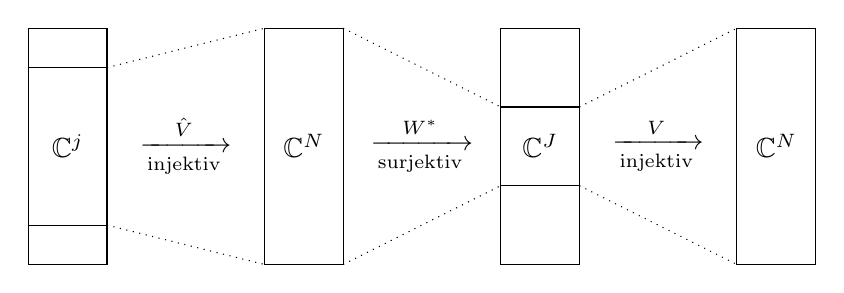
\begin{tikzpicture}[scale = 0.5]

        \draw (0,  0) rectangle (2,  6);
        \draw (6,  0) rectangle (8,  6);
        \draw (12, 0) rectangle (14, 6);
        \draw (18, 0) rectangle (20, 6);

        \draw (0, 1) -- (2, 1);
        \draw (0, 5) -- (2, 5);

        \draw [dotted] (2, 1) -- (6, 0);
        \draw [dotted] (2, 5) -- (6, 6);

        \draw [dotted] (8, 0) -- (12, 2);
        \draw [dotted] (8, 6) -- (12, 4);

        \draw (12, 2) -- (14, 2);
        \draw (12, 4) -- (14, 4);

        \draw [dotted] (14, 2) -- (18, 0);
        \draw [dotted] (14, 4) -- (18, 6);

        \draw (1,  3) node {$\C^j$};
        \draw (4,  3) node {$\xrightarrow[\text{injektiv}]{\hat V}$};
        \draw (7,  3) node {$\C^N$};
        \draw (10, 3) node {$\xrightarrow[\text{surjektiv}]{W^\ast}$};
        \draw (13, 3) node {$\C^J$};
        \draw (16, 3) node {$\xrightarrow[\text{injektiv}]{V}$};
        \draw (19, 3) node {$\C^N$};

    \end{tikzpicture}
    \caption{}
    \label{fig:rang_1}
\end{figure}

Matrizen haben genau dann denselben Rang, wenn sie äquivalent sind.

\begin{align*}
    \begin{pmatrix}
        \diag(\sigma_1, \dots, \sigma_J, \dots, \sigma_j) \\
        0_{(N - j) \times j}
    \end{pmatrix}
    =
    \Sigma
    \equiv
    \tilde V \Sigma \tilde W^\ast
    =
    A_0
    \equiv
    \begin{pmatrix}
        I_J \enspace 0_{J \times (j - J)} \\ 0_{(N - J) \times j}
    \end{pmatrix}
\end{align*}

Damit verschwinden die letzten Singulärwerte $\sigma_{J+1} = \cdots = \sigma_j = 0$.
Somit können wir statt der vollen Singulärwert-Zerlegung (indiziert mit \Quote{full}) eine reduzierte (indiziert mit \Quote{reduced}) verwenden.

\begin{align*}
    A_0
    =
    \tilde V_\mathrm{full} \Sigma_\mathrm{full} \tilde W_\mathrm{full}^\ast
    =
    \begin{pmatrix}
        \tilde V_\mathrm{reduced} & \ast
    \end{pmatrix}
    \begin{pmatrix}
        \Sigma_\mathrm{reduced} & 0_{J \times (j - J)}       \\
        0_{(N - J) \times J}    & 0_{(N - J) \times (j - J)}
    \end{pmatrix}
    \begin{pmatrix}
        \tilde W_\mathrm{reduced}^\ast \\ \ast
    \end{pmatrix}
    =
    \tilde V_\mathrm{reduced} \Sigma_\mathrm{reduced} \tilde W_\mathrm{reduced}^\ast
\end{align*}

Die $\tilde V_\mathrm{full}$ und $\tilde W_\mathrm{full}$ sind ja unitär, d.h. ihre Adjungierten waren ihre Inversen.

\begin{align*}
    \implies
    I_{N \times N}
    =
    \tilde V_\mathrm{full}^\ast \tilde V_\mathrm{full}
    =
    \begin{pmatrix}
        \tilde V_\mathrm{reduced}^\ast \\ \ast
    \end{pmatrix}
    \begin{pmatrix}
        \tilde V_\mathrm{reduced} & \ast
    \end{pmatrix}
    =
    \begin{pmatrix}
        \tilde V_\mathrm{reduced}^\ast \tilde V_\mathrm{reduced} & \ast \\
        \ast                                                     & \ast
    \end{pmatrix}
\end{align*}

Eine analoge Rechnung kann man, mit $j$ anstelle von $N$, für $\tilde W_\mathrm{reduced}$ machen.
Insgesamt erhalten wir also folgende Tatsachen über unsere reduzierte Singulärwert-Zerlegung.
Wir vereinbaren, ab sofort nur noch die reduzierte Singulärwert-Zerlegung zu verwenden und den Index wegzulassen.

\begin{align} \label{eq:singulärwert_zerlegung}
    \tilde V^\ast \tilde V
    =
    \tilde W^\ast \tilde W
    =
    I_{J \times J},
    \quad
    \Sigma = \diag(\sigma_1, \dots, \sigma_J),
    \quad
    A_0 = \tilde V \Sigma \tilde W^\ast
\end{align}

$\tilde V$ hat, als Teil-Matrix einer unitären, vollen Spaltenrang $J$ hat.
$\tilde V^\ast$ hat also vollen Zeilenrang $J$.
Abbildung \ref{fig:rang_2} illustriert, dass $S := \tilde V^\ast V \in \C^{J \times J}$ genau $J$ linear unabhängige Spalten hat, also $S \in \GL_J(\C)$.

\begin{figure}[!ht]
    \centering
    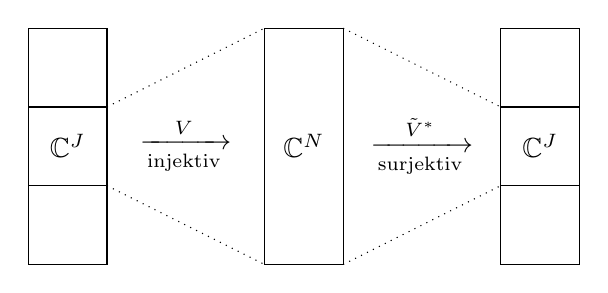
\begin{tikzpicture}[scale = 0.5]

        \draw (0,  0) rectangle (2,  6);
        \draw (6,  0) rectangle (8,  6);
        \draw (12, 0) rectangle (14, 6);

        \draw (0, 2) -- (2, 2);
        \draw (0, 4) -- (2, 4);

        \draw [dotted] (2, 2) -- (6, 0);
        \draw [dotted] (2, 4) -- (6, 6);

        \draw [dotted] (8, 0) -- (12, 2);
        \draw [dotted] (8, 6) -- (12, 4);

        \draw (12, 2) -- (14, 2);
        \draw (12, 4) -- (14, 4);

        \draw (1,  3) node {$\C^J$};
        \draw (4,  3) node {$\xrightarrow[\text{injektiv}]{V}$};
        \draw (7,  3) node {$\C^N$};
        \draw (10, 3) node {$\xrightarrow[\text{surjektiv}]{\tilde V^\ast}$};
        \draw (13, 3) node {$\C^J$};

    \end{tikzpicture}
    \caption{}
    \label{fig:rang_2}
\end{figure}

In den folgenden Gleichungsketten wird bei \Quote{!} die jeweils vorgerige eingesetzt.

\begin{align*}
    & \implies
    \Sigma \tilde W^\ast
    \stackrel
    {
        \eqref{eq:singulärwert_zerlegung}
    }{=}
    \tilde V^\ast \tilde V \Sigma \tilde W^\ast
    \stackrel
    {
        \eqref{eq:singulärwert_zerlegung}
    }{=}
    \tilde V^\ast A_0
    \stackrel
    {
        \eqref{eq:integral_matrizen_resultat}
    }{=}
    \tilde V^\ast V W^\ast \hat V
    =
    S W^\ast \hat V \\
    & \implies
    A_1
    \stackrel
    {
        \eqref{eq:integral_matrizen_resultat}
    }{=}
    V D W^\ast \hat V
    \stackrel{!}{=}
    V D S^{-1} \Sigma \tilde W^\ast \\
    & \implies
    \tilde V^\ast A_1 \tilde W \Sigma^{-1}
    \stackrel{!}{=}
    \tilde V^\ast V D S^{-1} \Sigma \tilde W^\ast \tilde W \Sigma^{-1}
    =
    S D S^{-1}
    \approx
    D
\end{align*}

Somit ist die Diagonalmatrix $D$, welche ja die gesuchten Eigenwerte enthält, ähnlich zur Matrix $\tilde V^\ast A_1 \tilde W \Sigma^{-1}$.
Ähnliche Matrizen haben dieselben Eigenwerte.

\subsection*{Zusammenfassung}

Wir haben insgesamt den folgenden Algorithmus \ref{alg:integral_methode_zusammenfassung} gefunden.

\begin{algorithm}[H]
	\label{alg:integral_methode_zusammenfassung}
	\caption{Integral-Methode}
    \begin{algorithmic}[1]
        \Procedure{Integral-Methode Zusammanfassung}{}
            \State Berechne $A_0, A_1 \in \C^{N \times j}$ (z.B. mit LU-Zerlegung);
            \State Berechne und reduziere eine Singulärwert-Zerlegung $A_0 = \tilde V \Sigma \tilde W^\ast$ auf $J$ Singulärwerte;
            \State Berechne Eigenwerte $\lambda_1, \dots, \lambda_k$ der Matrix $\tilde V A_1 \tilde W \Sigma^{-1}$ (z.B. mit QR-Verfahren);
            \State \Return $\lambda_1, \dots, \lambda_k$
		\EndProcedure
	\end{algorithmic}
\end{algorithm}

% % -------------------------------------------------------------------------------- %

\begin{exercise}

Zeigen Sie, dass für alle $n \geq 1$ gilt:
$(n! + 1, (n+1)! + 1) = 1$.

\end{exercise}

% -------------------------------------------------------------------------------- %

\begin{solution}

Um eine erste Idee zur Lösung zu erhalten, betrachten wir
zuerst einige Beispiele für kleine $n$:

\begin{align*}
  n &= 1: (2, 3) = 1 \\
  n &= 2: (3, 7) = 1 \\
  n &= 3: (7, 25) = (7, 5 \cdot 5) = 1 \\
  n &= 4: (25, 121) = (5 \cdot 5, 11 \cdot 11) = 1 \\
  n &= 5: (121, 721) = (11 \cdot 11, 7 \cdot 103) = 1
\end{align*}

Sei nun angenommen, dass $d := (n! + 1, (n+1)! + 1)  > 1$.

Da $(n+1)! + 1 - (n! + 1) = n!\cdot n$ folgt $d | n! \cdot n$.

Nun unterscheiden wir zwei Fälle:

\begin{itemize}
  \item[$(d,n) = 1$:] In dem Fall erhalten wir direkt $d | n!$ und 
  mit $d | (n! + 1 - n!) = 1$ einen Widerspruch!
  \item[$(d,n) > 1$:] In diesem Fall folgt aus $(d,n) | d$ und $d | n! + 1$, 
  sowie $(d,n) | n$ und $n | n!$,
  dass $(d,n) | (n! + 1 - n!) = 1$ mit Widerspruch zu $(d,n) > 1$!
\end{itemize}

\end{solution}

% -------------------------------------------------------------------------------- %

% % -------------------------------------------------------------------------------- %

\begin{exercise}[Legendre]

Zeigen Sie, dass die Zahl $n!$ den Primfaktor $p$ genau

\begin{align*}
  \sum_{k \geq 1} \left\lfloor \frac{n}{p^k}\right\rfloor
\end{align*}
Mal enthält.
\end{exercise}

% -------------------------------------------------------------------------------- %

\begin{solution}

Die Zahl $n!$ enthält den Primfaktor $p$ genau $\sum_{i=1}^n \nu_p(i)$ Mal.
Die Zahlen bis $n$, welche den Primfaktor $p$ mindestens einmal enthalten sind genau
$p,2p,\dots,\left\lfloor \frac{n}{p}\right\rfloor p$.
Ebenso gibt es genau $\left\lfloor \frac{n}{p^k}\right\rfloor$ Zahlen bis $n$,
welche den Primfaktor $p$ mindestens $k$ Mal enthalten. \\
Damit erhalten wir mit $\sum_{k \geq 1} \left\lfloor \frac{n}{p^k}\right\rfloor$
genau die Anzahl, wie oft der Primfaktor $p$ in $n!$ enthalten ist.

\end{solution}

% -------------------------------------------------------------------------------- %

% \begin{exercise}

Sei $X$ ein topologischer Vektorraum.
Eine Menge $B \subseteq X$ heißt beschränkt, falls es zu jeder Nullumgebung $U$ ein positive Zahl $\lambda_U$ gibt, sodass $B \subseteq \lambda_U U$.
Zeige, dass jede kompakte Teilmenge von $X$ beschränkt ist. Zeige, dass jeder lineare Teilraum $Y \neq \Bbraces{0}$ von $X$ unbeschränkt ist.

\end{exercise}

\begin{solution}

Trivial!

\end{solution}

% \begin{exercise}

Sei $X$ ein topologischer Vektorraum und $B \subseteq X$.
Zeige, dass die folgenden Aussagen äquivalent sind:

\begin{enumerate}[label = (\roman*)]
  \item $B$ ist beschränkt.
  \item Zu jeder Nullumgebung $U$ gibt es eine Zahl $\mu_U > 0$, sodass $B \subseteq \lambda U$ für alle $\lambda > \mu_U$.
  \item Für jede Folge $(x_n)_{n \in \N}$ von Elementen von $B$ und jede Folge $(\alpha_n)_{n \in \N}$ komplexer Zahlen mit $\lim_{n \to \infty} \alpha_n = 0$ gilt $\lim_{n \to \infty} \alpha_n x_n = 0$.
\end{enumerate}

\end{exercise}

\begin{solution}

\Quote{(i) $\Rightarrow$ (ii)}:
Seien $W, U \in \mathfrak{U}(0)$, mit $W \subseteq U$ kreisförmig.
Nachdem $B$ beschränkt ist, $\Exists \mu_U > 0: \Forall \lambda > \mu_U:$

\begin{align*}
  B
  \subseteq
  \mu_U W
  \stackrel{!}{\subseteq}
  \lambda W
  \subseteq
  \lambda U.
\end{align*}

Dabei gilt \Quote{!}, weil $|\frac{\mu_u}{\lambda}| \leq 1$ und somit $\frac{\mu_u}{\lambda} W \subseteq W$, da $W$ kreisförmig ist. \\

\Quote{(ii) $\Rightarrow$ (i)}:
Trivial! \\

\Quote{(i) $\Rightarrow$ (iii)}:
Sei $U \in \mathfrak{U}(0)$ kreisförmig, und $(x_n) \in B$.
Weil $B$ beschränkt ist, $\Exists \lambda > 0: (x_n) \in B \subseteq \lambda U$.
Wenn nun $(\alpha_n) \in \C$, mit $\alpha_n \to 0$, dann gilt für fast alle $n \in \N:$

\begin{align*}
  |\alpha_n| \leq \frac{1}{\lambda}
  \Rightarrow
  \frac{x_n}{\lambda} \in U,
  |\alpha_n \lambda| \leq 1
  \Rightarrow
  \alpha_n x_n \in U.
\end{align*}

\Quote{(iii) $\Rightarrow$ (i)}:
Angenommen, $\Exists U \in \mathfrak{U}(0): \Forall \lambda > 0: B \not \subseteq \lambda U$, d.h. $\Exists x_\lambda \in B: x_\lambda \notin \lambda U$.
Sei nun $(\alpha_n) \in \R^+: \alpha_n \to 0$ und definiere $\lambda_n := \frac{1}{\alpha_n}$.
Weil $B$ ja nicht beschränkt ist, muss $\Forall n \in \N: \Exists x_n \in B:$

\begin{align*}
  x_n \notin \lambda_n U
  \Rightarrow
  \alpha_n x_n \notin U.
\end{align*}

Somit $\Exists (x_n) \in B, \Exists (\alpha_n) \in \C: \alpha_n \to 0, \alpha_n x_n \not \to 0$, d.h. $\Exists U \in \mathfrak{U}(0): \Forall N \in \N: \Exists n \geq N: \alpha_n x_n \notin U$.

\end{solution}


\end{document}
